%\documentclass[xcolor={dvipsnames}, handout]{beamer}
\documentclass[xcolor={dvipsnames}]{beamer}
\setbeamertemplate{footline}[frame number]
\setbeamersize{description width=-\labelsep}

%\usepackage{amsmath,amsfonts,amssymb,pxfonts,eulervm,xspace}
\usepackage{amsmath, amsfonts, amssymb, mathtools, eulervm, xspace}
\renewcommand{\restriction}{\mathord{\upharpoonright}} %restriction w/p space
\usepackage{relsize} %mathlarger
\usepackage{bm}
\usepackage{centernot}
\usepackage{mathrsfs} % math script fonts
\usepackage{tikz}
\usetikzlibrary{cd} % commutative diagrams
\newtheorem{prop}{Proposition} %math?

\usepackage{subcaption} % subfigure float captioning

\usepackage{tabulary}
\usepackage{tabularx}
%\usepackage{enumitem} $ won't work with beamer
\usepackage{booktabs}
\usepackage{multirow}
\usepackage{array}

\usepackage{graphicx}
\usepackage{adjustbox}%scale tikz-cd

\usepackage{appendixnumberbeamer} 
\usepackage{comment}
\usepackage{minted}
\setminted[python]{fontsize=\scriptsize, 
                   linenos,
                   numbersep=8pt,
                   autogobble, 
                   frame=lines,
                   bgcolor=bg,
                   framesep=3mm} 

\usepackage{notation} % move this later

\graphicspath{.figures/}

\usepackage[backend=bibtex, sorting=none, doi=false,isbn=false,url=false, giveninits=true]{biblatex}
\bibliographystyle{plain}
\bibliography{../paper/bibliography.bib}

%\usetheme{ccnycrest}

\newenvironment{changemargin}[2]{%
\begin{list}{}{%
\setlength{\topsep}{0pt}%
\setlength{\leftmargin}{#1}%
\setlength{\rightmargin}{#2}%
\setlength{\listparindent}{\parindent}%
\setlength{\itemindent}{\parindent}%
\setleng{}th{\parsep}{\parskip}%
}%
\item[]}{\end{list}}

\begin{document}
\begin{frame}<presentation:1-|handout:0>{About}
    Slides: https://bit.ly/team329
    \begin{block}{Me (twitter/github: story645)}
        \begin{itemize}
            \item nth year grad student (on my 3rd EO)
            \item former adjunct at CCNY, former Digital Fellow
            \item Matplotlib Community Manager \& Core Developer
        \end{itemize}
    \end{block}

    \begin{block}<presentation:2|handout:0>{Project}
        \begin{itemize}
            \item Funded by Chan Zuckerberg Initiative EOSS 1 \& 3
            \item paper rejected by vizweek last spring
            \item work has since gone all in on category theory 
        \end{itemize}
    \end{block}
\end{frame}

\begin{frame}<presentation:1|handout:1>
	\titlepage
    Hannah Aizenman, Tom Caswell, Michael Grossberg\\
    %Committee: Dr. Robert Haralick, Dr. Lev Manovich, Dr. Huy Vo\\
    %External Member: Dr. Marcus Hanwell
\end{frame}

\section{Introduction}
\begin{frame}<presentation:0|handout:0>{What are we doing?}
    \begin{itemize}
        \item develop a model for describing data to graphic transformations
        \item specify a visualization library architecture based on this model
        \item implement functional(ish) components based on this model using ideas from functional programming
    \end{itemize}
\end{frame}


%% maybe pull out the middle for now? move the 3 stages down to construction? 
\begin{frame}<presentation:1-|handout:0>{What do visualization libraries do?}
    \begin{figure}
        \begin{overprint}
            \onslide<1|handout:1>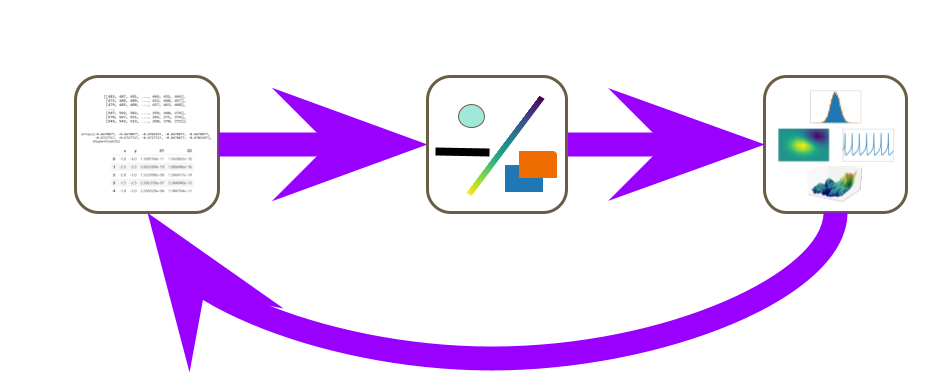
\includegraphics[width=\linewidth]{figures/flow/s2.png}
            \onslide<2|handout:2>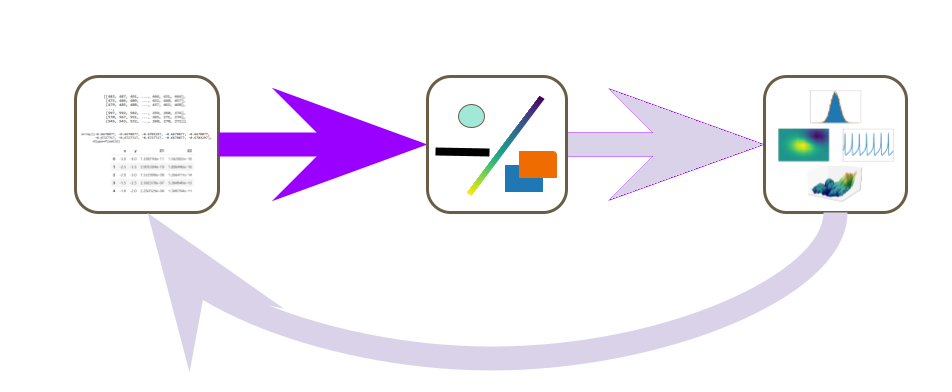
\includegraphics[width=\linewidth]{figures/flow/s_vc.png}
            \onslide<3|handout:3>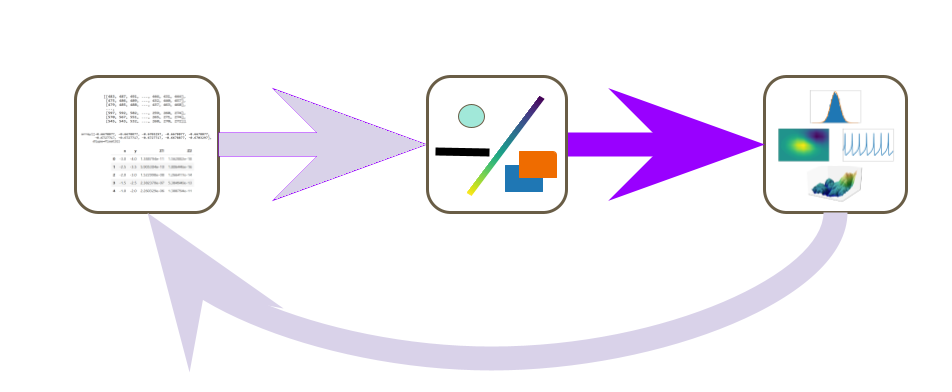
\includegraphics[width=\linewidth]{figures/flow/s_mark.png}
            \onslide<4|handout:4>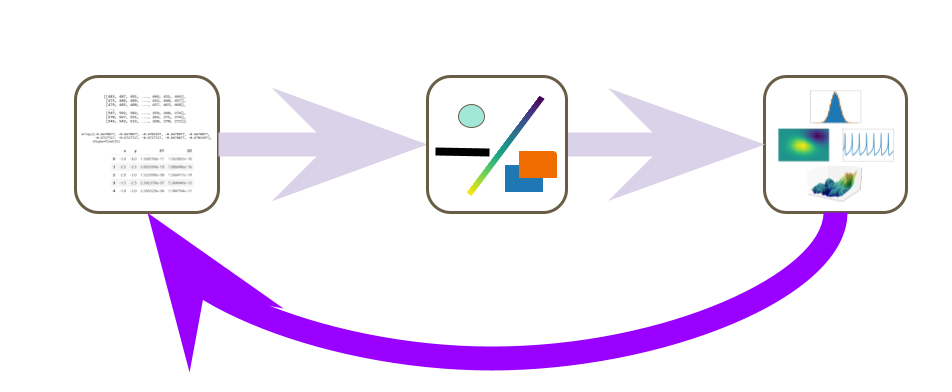
\includegraphics[width=\linewidth]{figures/flow/s3.png}
        \end{overprint}
    \end{figure}
\end{frame}



\begin{frame}<presentation:1|handout:0>{Matplotlib}
    \begin{figure}
       
\includegraphics[width=\linewidth]{figures/flow/artists.png}
    \end{figure}
\end{frame}


\begin{frame}<presentation:1-|handout:0>
    \frametitle<presentation:1-2|handout:0>{Everything is an Artist}
    \frametitle<presentation:3|handout:0>{Transformations Change Artists into Different Coordinates}
    \begin{overprint}
        \onslide<1|handout:0>\includegraphics[scale=.25]{figures/math/sphx_glr_anatomy_001_2_0x.png}
        \onslide<2|handout:0>\includegraphics[width=\textwidth]{figures/math/artist_tree.png}
        \onslide<3|handout:0>\includegraphics[width=\textwidth]{figures/math/transforms.png}
    \end{overprint}
\end{frame}


\begin{frame}[fragile]{A Simple Artist}
\begin{minted}{python}
    class SomeArtist(Artist):
        'An example Artist that implements the draw method'
    
        def draw(self, renderer):
            # create some objects and use renderer to draw self here
            renderer.draw_path(graphics_context, path, transform)
\end{minted}
\end{frame}

\begin{frame}<presentation:1-|handout:0>{Goals}
    \begin{figure}
        
\includegraphics[width=\linewidth]{figures/flow/artists.png}
    \end{figure}
\end{frame}

\begin{frame}<presentation:1|handout:0>{How do we express structure?} 
    \begin{figure}
        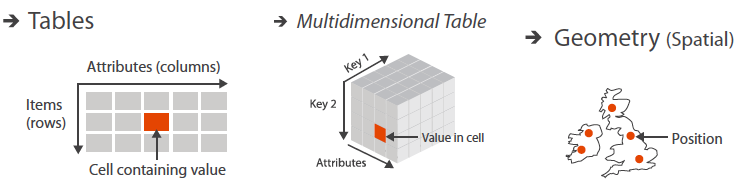
\includegraphics[width=1\textwidth]{figures/intro/munzner_datatypes.png}
        \caption{Figure 2.8 in Munzner's Visualization Analysis and Design\cite{munznerVisualizationAnalysisDesign2014}}
    \end{figure}
\end{frame}

\begin{frame}<presentation:1|handout:0>{Continuity}
    \begin{figure}
        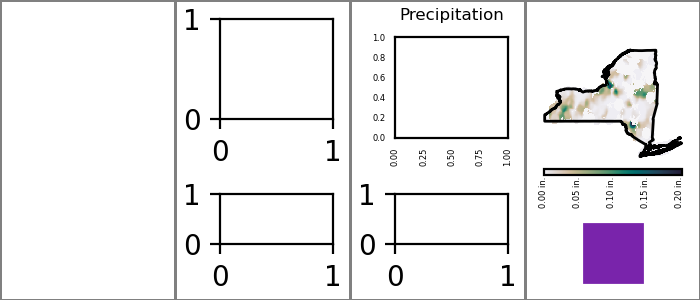
\includegraphics[width=\linewidth]{../paper/figures/k_different_types.png}
    \end{figure}
    \begin{block}{Topological Properties \cite{wilkinsonGrammarGraphics2005}}
        how elements in a dataset are organized, e.g. discrete rows in a table, networked nodes, pixels in an image, points on a line
    \end{block}
\end{frame}

\begin{frame}<presentation:1|handout:0>{Visual Algorithms \& Continuity}
    \begin{figure}
        \includegraphics[width=1\linewidth]{figures/math/plottypes.png}
    \end{figure}
\end{frame}

\begin{frame}<presentation:1-|handout:0>{Equivariance}
    \begin{description}
        \item[What] Retinal Variables \& Marks: visual encodings should match properties of the data \cite{bertinSemiologyGraphicsDiagrams2011a}
        \pause
        \item[Why] Graphical Integrity: graphs show \textbf{only} the data\cite{tufteVisualDisplayQuantitative2001}
        \pause 
        \item[Why] Naturalness: easier to understand when properties match\cite{norman_things_smart}
        \pause
        \item[How] Expressiveness: which structure preserving mappings can a tool implement\cite{mackinlayAutomatingDesignGraphical1986}] 
    \end{description}
\end{frame}

%flip columns
\begin{frame}<presentation:0-|handout:0>{Theoretical Frameworks}
    \begin{description}
        \item[linguistically] visualization has syntax, semantics, grammar expresses how to design structure preserving visualizations
        \cite{mackinlayAutomatingDesignGraphical1986,mackinlayAUTOMATICDESIGNGRAPHICAL1987,wilkinsonGrammarGraphics2005}

        \item[algebraically] transformations on data and graphics are equivalent and symmetric \cite{kindlmannAlgebraicProcessVisualization2014}
        \begin{columns}
            \column{.5\textwidth}
            \begin{description}
                \item[D] raw data 
                \item[R] representation (data container) 
                \item[V] visualization
            \end{description}
            \column{.5\textwidth}
            \begin{equation*}
                \begin{tikzcd}[ampersand replacement=\&]
                    D \arrow[d, "\alpha"'] \arrow[r, "r_1"] \& R \arrow[r, "\nu"]  \& V \arrow[d, "\omega"] \\
                    D \arrow[r, "r_2"']                     \& R \arrow[r, "\nu"'] \& V                    
                \end{tikzcd}
            \end{equation*}
        \end{columns} 
    %\item[categorically] \textit{understanding} = \textit{read} $\circ$ \textit{render} \cite{vickersUnderstandingVisualizationFormal2013}    
    \end{description}
\end{frame}

\begin{frame}<presentation:1-|handout:1>
    \frametitle{Domain Specific Library: library assumes structure \cite{HeerSoftware2006}}
    \begin{table}
        %\renewcommand{\arraystretch}{2}
        %
        \begin{tabular}{>{\onslide<1->}l>{\onslide<2->}l>{\onslide<3->}l}
            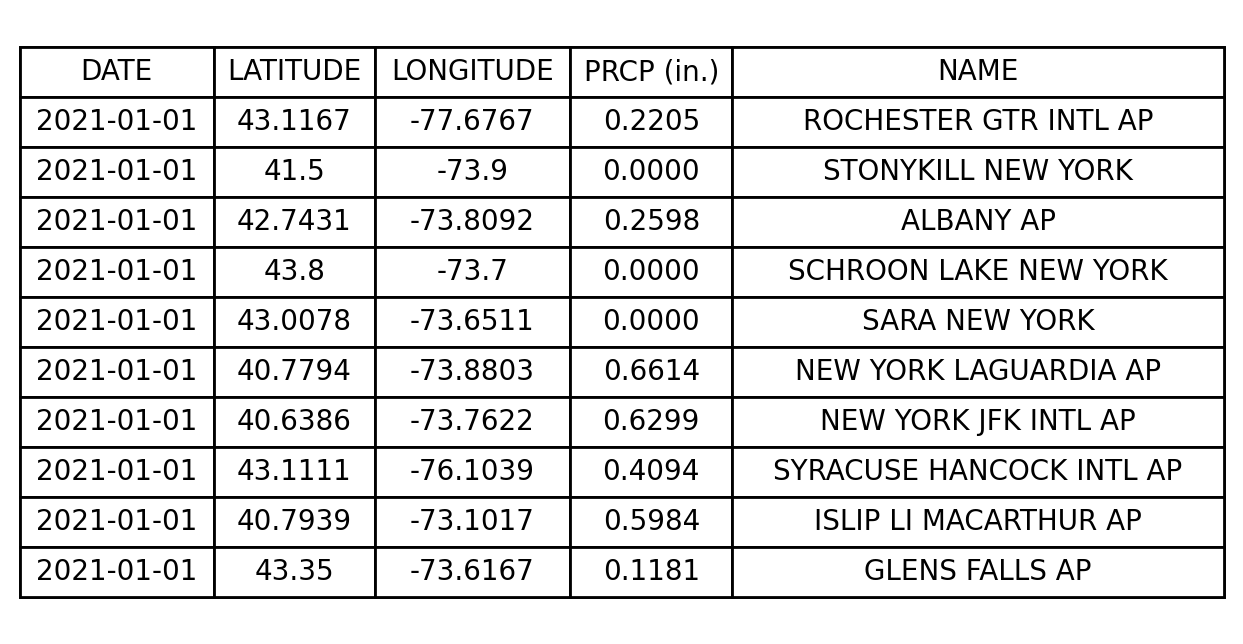
\includegraphics[width=.24\textwidth]{figures/intro/table.png} & 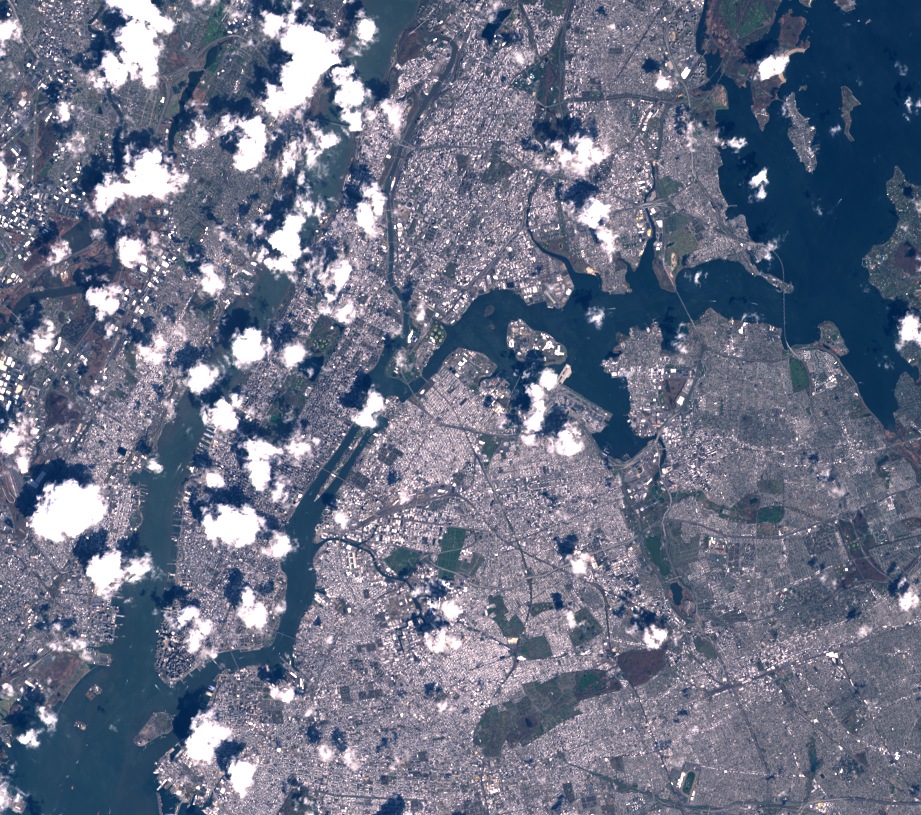
\includegraphics[width=.3\textwidth]{figures/intro/landsat.png} & 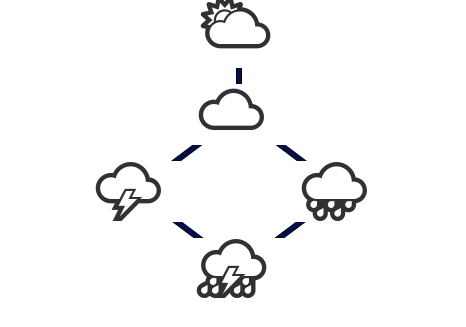
\includegraphics[width=.33\textwidth]{figures/math/graph.png} \\
            ggplot\cite{wickhamGgplot2ElegantGraphics2016a}  & ImageJ\cite{schneiderNIHImageImageJ2012}& Gephi\cite{bastianGephiOpenSource2009}\\
            Vega\cite{satyanarayanDeclarativeInteractionDesign2014} & ImagePlot\cite{studiesCulturevisImageplot2021} & Graphviz\cite{ellsonGraphvizOpenSource2002}\\
            Altair\cite{vanderplasAltairInteractiveStatistical2018}& Napari\cite{nicholas_sofroniew_2021_4533308} & Networkx\cite{HagbergExploringNetwork2008}\\
             Tableau \cite{StoltePolaris2002}& &\\
            \cite{hanrahanVizQL2006,MackinlayShowme2007}&&\\        
        \end{tabular}
    \end{table}
\end{frame}

\begin{frame}<presentation:1-|handout:1>
    \frametitle{Building Block Library\cite{wongsuphasawatNavigatingWideWorld2021}: visual algorithms assume structure \cite{toryRethinkingVisualizationHighlevel2004}}
    \begin{figure}
        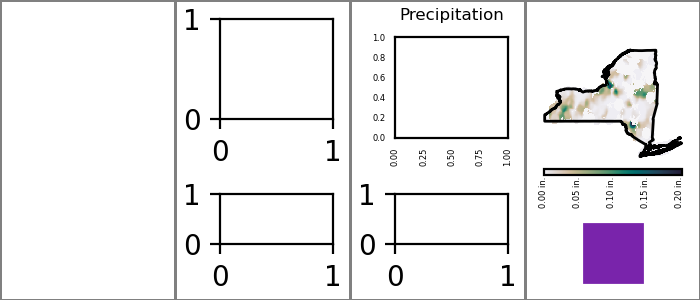
\includegraphics[height=.3\textheight]{../paper/figures/k_different_types.png}
    \end{figure}

    \begin{enumerate}
        \item Matplotlib\cite{hunterMatplotlib2DGraphics2007} $\rightarrow$ Seaborn\cite{waskom2020seaborn}, xarray \cite{hoyer2017xarray} 
        \item D3 \cite{bostockDataDrivenDocuments2011}
        \item VTK \cite{hanwellVisualizationToolkitVTK2015,geveciVTK2012},MayaVi\cite{RamachandranMayaVI2011}$\rightarrow$ Titan\cite{brianwylieUnifiedToolkitInformation2009}, ParaView\cite{ahrens2005paraview}
    \end{enumerate}
\end{frame}

\section{Algebraic Topology & Category Theory}
\begin{frame}<presentation:1|handout:1>{Design Composable Structure Preserving API}
    \begin{description}
        \item[Fiber Bundles] "unified, dimension-independent framework" that expresses data as the mapping between continuity and fields \cite{butlerVectorBundleClassesForm1992,butlerVisualizationModelBased1989}
        \item[Category Theory Language] express constraints in specifications \cite{wielsManagementEvolvingSpecifications1998}   
        \item[Sheaves on Bundles] "algebraic data structure" for representing data over topological spaces \cite{ghristElementaryAppliedTopology2014}
    \end{description}
\end{frame}

\subsection{Fiber Bundles}
\begin{frame}<presentation:1-|handout:1>
    \frametitle<1|handout:1>{Fiber Bundle}
    \frametitle<6|handout:2-3>{Data Bundle}
    \frametitle<7|handout:4-5>{Graphic Bundle}
    \begin{columns}
        \column{0.31\textwidth}
        \begin{equation*}
            %\label{eq:related-work:continuity:fiber-bundle}
            \begin{tikzcd}[ampersand replacement=\&, row sep=huge]
              \onslide*<3-6|handout:1-2>{\dfiberc}
              \onslide*<7|handout:4>{\gfiberc} 
              \onslide*<4-|handout:1-2,4>{\arrow[r, hook]} \& 
              \onslide*<1-6|handout:1-2>{\dtotalc} 
              \onslide*<7|handout:4>{\gtotalc}
              \onslide*<4-|handout:1-2,4>{\arrow[d, "\pi"']} \\
               \& 
               \onslide*<2-6|handout:1-2>{\dbasec}
               \onslide*<7|handout:4>{\gbasec} 
               \onslide*<5-6|handout:1-2>{\arrow[u, "\dsectionc"', bend right, pos=.5]}
               \onslide*<7|handout:4>{\arrow[u, "\gsectionc"', bend right, pos=.5]}
            \end{tikzcd}
        \end{equation*}
     \column{0.69\textwidth}
     \only<1-5|handout:1>{
        \begin{description}
            \item<1-5|handout:1>[\textcolor{total}{Total Space}]{$(\dtotalc, \mathcal{T}_{\dtotalc})$}
            \item<2-5|handout:1>[\textcolor{base}{Base Space}]{$(\dbasec, \mathcal{T}_{\dbasec}),\; \dbasepointc \in \opensetc \subseteq \dbasec$}
            \item<3-5|handout:1>[\textcolor{fiber}{Fiber Space}]{$\dfiberc\restriction_{\dbasepointc} = \pi^{-1}(\dbasepointc), \dfiberc = \dfiberc\restriction_{\dbasepointc}\; \forall \dbasepointc \in \dbasec$}
        \end{description}
        }
    \only<6|handout:2>{
        \begin{description}
            \item[\textcolor{total}{Data \dtotalc}]{continuity + fields}
            \item[\textcolor{base}{Continuity \dbasec}]{how data elements are organized (topological properties) \cite{wilkinsonGrammarGraphics2005}, index (key) space \cite{munznerWhatDataAbstraction2014})}
            \item[\textcolor{fiber}{Fields \dfiberc}] {generalization of a schema - named and typed date fields \cite{spivakSIMPLICIALDATABASES, spivakDatabasesAreCategories2010}}
        \end{description}
        }
        \only<7|handout:4>{
            \begin{description}
                \item[\textcolor{total}{Graphic \gtotalc}]{continuity + renderer fields}
                \item[\textcolor{base}{Continuity \gbasec}]{parameterization of graphic area (e.g. "inked" bounding box\cite{CairographicsOrg})}
                \item[\textcolor{fiber}{Display \gfiberc}] {renderer fields, e.g. \{xy,rgba\}, \{xy, cymk\}, \{xyz, rgba\}}
            \end{description}
            }
    \end{columns}
    \only<4-5|handout:1>{
        \begin{alertblock}{}
            \begin{description}
                \only<5:handout:1>{\item[\textcolor{section}{Sections}]{$\cgamma{\opensetc}{\dtotalc\restriction_{\opensetc}} \coloneqq \big\{\dsectionc: \opensetc\rightarrow \dtotalc\restriction_{\opensetc} \; \bigm{\vert} \pi(\dsectionc(\dbasepointc)) = \dbasepointc\;for\, all\; \dbasepointc \in \opensetc \big\}$}}
            \end{description}
        \end{alertblock}
    }
    \only<4:handout:1>{
        \begin{alertblock}{}
    \begin{description}
    \item[Locally Trivial] {for every point $\dbasepointc \in \dbasec$, there exists an open neighborhood $\dbasepointc \in \opensetc \subseteq \dbasec$ s.t. there is a homeomorphism $\pi^{-1}(\opensetc)\xrightarrow{\equivc} \opensetc \times \dfiberc$}
    \item[(Globally) Trivial]{$\dtotalc = \dbasec \times \dfiberc$}
\end{description}
\end{alertblock}
    }
    \only<6|handout:2>{
    \begin{alertblock}{}
        \begin{description}
            \item[\textcolor{section}{Data} \cite{butlerVisualizationModelBased1989,butlerVectorBundleClassesForm1992}]{$
        \dsectionc(\dbasepointc) = \;\delementc,\; \dbasepointc\in \opensetc \subseteq \dbasec,\; \delementc \in \dfiberc\restriction_{\dbasepointc}$} 
        \item[]{$\delementc=\{field_0:value, \cdots field_i:value, \cdots field_n:value\}$}
        \end{description}
    \end{alertblock}
    }
    \only<7|handout:4>{
        \begin{alertblock}{}
            \begin{description}
                \item[\textcolor{section}{Graphic}]{$\cgamma{\opensetgc}{\gtotalc\restriction_{\opensetgc}} \coloneqq \big\{\gsectionc: \opensetgc\rightarrow \gtotalc\restriction_{\opensetgc} \; \bigm{\vert} \pi(\gsectionc(\gbasepointc)) = \gbasepointc\;for\, all\; \gbasepointc \in \opensetgc \big\}$}
                \item[] {$\gsectionc(\gbasepointc) = \gelementc,\; \gbasepointc\in \opensetgc\subseteq \gbasec,\; \gelementc \in \dfiberc\restriction_{\gbasepointc}$}
                \item[] $\gelementc=\{x,\,y,\,r,\,g,\,b\}$
           
        \end{description}    
    \end{alertblock}
    }
    \only<|handout:3>{
        \begin{figure}
            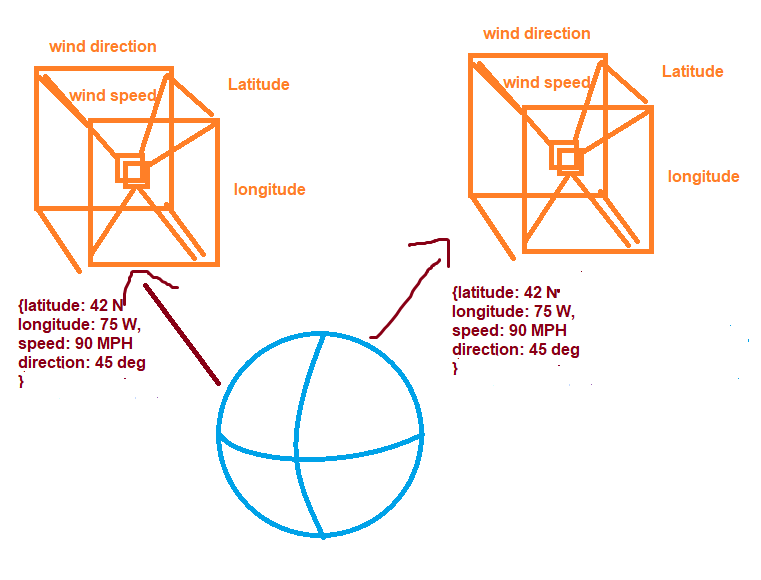
\includegraphics[scale=.65]{figures/math/spherebundle.png}
        \end{figure}
    }
    \only<|handout:5>{
        \begin{figure}
            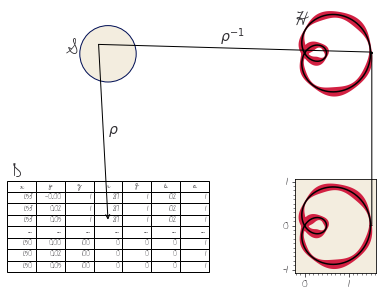
\includegraphics[scale=.65]{figures/math/render.png}
        \end{figure}
    }
\end{frame}

\subsection{Category Theory Language}
\begin{frame}<presentation:1|handout:1>[fragile]{}
    \begin{minted}{python}
        Artist(Data) -> Graphic
    \end{minted}
\end{frame}

\begin{frame}<presentation:1-|handout:1->
    \frametitle<presentation:1-6|handout:1>{Category \setc}
    \frametitle<presentation:7|handout:2>{Category \setc^{op}}
\begin{columns}
    \column{0.39\textwidth}
    \begin{equation*}
    \begin{tikzcd}[ampersand replacement=\&]
        \onslide*<1-|handout:1>{\setc_1} 
        \onslide*<3-6|handout:1>{\arrow[r, "r_{1,2}", color=set]}
        \onslide*<4-6|handout:1>{\arrow[rd, "r_{1,2}\circ r_{2,3}"', color=set]}
        \onslide*<2-6|handout:1>{\arrow["id_{\setc_1}"', loop, distance=2em, in=215, out=145, color=set]} \& 
        \onslide*<1-|handout:1>{\setc_2}
        \onslide*<7|handout:2>{\arrow[l, color=set]}
        \onslide*<3-6|handout:1>{\arrow[d, "r_{2,3}", color=set]} 
        \onslide*<2-6|handout:1>{\arrow["id_{\setc_2}"', loop, distance=2em, in=125, out=55, color=set]} \\\& 
        \onslide*<1-|handout:1>{\setc_3}
        \onslide*<7|handout:2>{\arrow[u, color=set]}
        \onslide*<7|handout:2>{\arrow[lu, color=set]}
        \onslide*<2-6|handout:1>{\arrow["id_{\setc_3}"', loop, distance=2em, in=305, out=235, color=set]}              
    \end{tikzcd}
    \end{equation*}
    \column{0.59\textwidth}
    \begin{alertblock}<5-6|handout:1>{associativity} 
        if $r_{1,2}: \setc_1 \rightarrow \setc_2$, $r_{2,3}: \setc_2 \rightarrow \setc_3$ and $r_{3,4}: \setc_3 \rightarrow \setc_4$ then $r_{3,4}\circ (r_{2,3} \circ r_{1,2}) = (r_{3,4} \circ r_{2,3}) \circ r_{1,2}$
    \end{alertblock}
    \begin{alertblock}<6|handout:1>{identity} 
        for every $r_{1,2}: \setc_1 \rightarrow \setc_2$ there exists identity morphisms $r_{1,2} \circ id_{\setc_1} = r_{1,2} = id_{\setc_2} \circ r_{1,2}$
    \end{alertblock}
    \end{columns}
\end{frame}


\begin{frame}<presentation:0|handout:1>{Opposite Category $\textcolor{source}{\mathcal{C}^{op}}$}
    \begin{columns}
        \column{0.49\textwidth}
    \begin{equation*}
        \begin{tikzcd}[ampersand replacement=\&]
            \textcolor{fade}{C_1} \arrow[r, "f", color=fade] \arrow[rd, "g\circ f"', color=fade] \arrow["id_{C_1}"', loop, distance=2em, in=215, out=145, color=fade] \& \textcolor{fade}{C_2} \arrow[d, "g", color=fade] \arrow["id_{C_2}"', loop, distance=2em, in=125, out=55, color=fade] \\
        \& \textcolor{fade}{C_3} \arrow["id_{C_3}"', loop, distance=2em, in=305, out=235, color=fade]              
        \end{tikzcd}
        \end{equation*}
        \column{0.49\textwidth}
        \onslide*<presentation:2|handout:1>{
        \begin{equation*}
        \begin{tikzcd}[ampersand replacement = \&]
            \textcolor{source}{C_1} \arrow["id_{C_1}"', loop, distance=2em, in=215, out=145, color=source] \& \textcolor{source}{C_2} \arrow[l, "f"',color=source] \arrow["id_{C_2}"', loop, distance=2em, in=125, out=55, color=source]\\
            \& \textcolor{source}{C_3} \arrow[u, "g"', color=source] \arrow[lu, "f \circ g", color=source] \arrow["id_{C_3}"', loop, distance=2em, in=305, out=235, color=source]
            \end{tikzcd}
        \end{equation*}
        }
        \end{columns}
\end{frame}

\begin{frame}<presentation:1-|handout:1>
    \frametitle{Functor $\textcolor{functor}{\bm{F}}: \textcolor{source}{\mathcal{C}} \rightarrow \textcolor{target}{\mathcal{D}}$}
\begin{columns}
    \column{.39\textwidth}
    \begin{equation*}
        \begin{tikzcd}[ampersand replacement = \&, ]
            \onslide*<1-|handout:1>{\textcolor{source}{c}} 
            \onslide*<1-|handout:1>{\arrow[d, "f"', shift right=0, color=source]} 
            \onslide*<3-|handout:1>{\arrow[r, "F", color=functor, maps to]} \& 
            \onslide*<2-3|handout:0>{\textcolor{target}{d}}
            \onslide*<4-|handout:0>{\textcolor{target}{F(c)}} 
            \onslide*<0|handout:1>{\textcolor{target}{F(c)=d}} 
            \onslide*<2|handout:0>{\arrow[d, shift right=0, color=target]}
            \onslide*<3-|handout:0>{\arrow[d, "F(f)", shift right=0, color=target]}
            \onslide*<0|handout:1>{\arrow[d, "F(f)", shift right=3, color=target]} \\
            \onslide*<1-|handout:1>{\textcolor{source}{c^{\prime}}} 
            \onslide*<3-|handout:1>{\arrow[r, "F"', color=functor, maps to]}\& 
            \onslide*<2-3|handout:0>{\textcolor{target}{d^{\prime}}}
            \onslide*<4-|handout:0>{\textcolor{target}{F(c^{\prime})}}
            \onslide*<0|handout:1>{\textcolor{target}{F(c^{\prime})= d^{\prime}}}                    
        \end{tikzcd}
    \end{equation*}
    \column{.59\textwidth}
    \begin{alertblock}<5-|handout:1>{composition}
        \begin{align*}
            \textcolor{functor}{F}(\textcolor{source}{g}) \circ  \textcolor{functor}{F}(\textcolor{source}{f}) = \textcolor{functor}{F} (\textcolor{source}{g}\circ \textcolor{source}{f})
        \end{align*}
    \end{alertblock}
    \begin{alertblock}<6-|handout:1>{identity}
        \begin{align*}
            \textcolor{functor}{F}(\textcolor{source}{id_c}) = \textcolor{target}{id}_{\textcolor{functor}{F}(\textcolor{source}{c})}
        \end{align*}
    \end{alertblock}
\end{columns}
\end{frame}

\subsubsection{Natural Transforms}
\begin{frame}<presentation:1-|handout:1>
    \frametitle{Natural Transformation $\textcolor{nattran}{\alpha}: \textcolor{functor}{F} \textcolor{nattran}{\Rightarrow} \textcolor{functor}{G}$}
    \adjustbox{scale=3, center}{
        \begin{tikzcd}[ampersand replacement=\&]
            \& {} \arrow[dd, "\alpha" , Rightarrow, shorten=1.5em, color=nattran] \&             \\
          \textcolor{source}{\mathcal{C}} \arrow[rr, "F", bend left, color=functor] \arrow[rr, "G"', bend right, color=functor] \& \& \textcolor{target}{\mathcal{D}} \\
            \& {} \&            
          \end{tikzcd}}
\end{frame}

\begin{frame}<presentation:1-|handout:1>
    \frametitle{Natural Transformation $\textcolor{nattran}{\alpha}: \textcolor{functor}{F} \textcolor{nattran}{\Rightarrow} \textcolor{functor}{G}$}
    \begin{equation*}
        \begin{tikzcd}[ampersand replacement=\&]  
                \&  \& 
                \textcolor{target}{d_s} \& 
                \textcolor{source}{c} 
                \arrow[r, "G", maps to, color=functor] 
                \arrow[l, "F"', maps to, color=functor] \& 
                \textcolor{target}{d_t} \\
                \textcolor{source}{c_1} 
                \arrow[dd, "f" description, color=source] \& \& 
                \textcolor{target}{F(c_1)} 
                \arrow[dd, "F(f)"', color=target] 
                \arrow[rr, "\alpha_{c_1}", color=nattran] \& \& 
                \textcolor{target}{G(c_1)} 
                \arrow[dd, "G(f)", color=target] \\
                \& \& {} 
                \arrow[rr, "\alpha_{f}", dotted, color=nattran] \& \& {} \\
                \textcolor{source}{c_2} \& \& 
                \textcolor{target}{F(c_2)} 
                \arrow[rr, "\alpha{c_2}", color=nattran] \& \& 
                \textcolor{target}{G(c_2)} \\
                \& \& 
                \textcolor{target}{F} 
                \arrow[rr, "\alpha", Rightarrow, color=nattran] \& \& 
                \textcolor{target}{G}                        
        \end{tikzcd}                    
    \end{equation*}
\end{frame}

\subsection{Sheaves}

\begin{frame}<presentation:1-|handout:1>
    \frametitle{Presheaf: $\sheafc: \mathcal{C}^{op} \textcolor{sheaf}{\rightarrow} \setc $}
    \begin{columns}
    \column{0.29\textwidth}
    \begin{tikzcd}[ampersand replacement=\&, row sep=huge]
        \onslide*<9-|handout:1->{\dfiberc}
        \onslide*<9-|handout:1->{\arrow[r, hook]} \& 
        \onslide*<1-|handout:1->{\dtotalc}
        \onslide*<1-|handout:1->{\arrow[d, "\pi"']} \\
           \& 
        \onslide*<1-|handout:1->{\dbasec}
        \onslide*<3-|handout:1->{\arrow[u, "\dsectionc \in \cgamma{\dbasec}{\dtotalc}"', bend right, pos=.5]}
        \end{tikzcd}
    \column{0.69\textwidth}
        \begin{tikzcd}[ampersand replacement = \&, column sep=small]
            \onslide*<3,6-|handout:0>{{\cgamma{\opensetc_1}{\dtotalc\restriction_{{\opensetc_1}}}}} 
            \onslide*<4-5|handout:0>{{\cgamma{\opensetc_1}{\dtotalc\restriction_{{\opensetc_1}}}}\in Ob(\setc)}
            \onslide*<0|handout:1>{\Ob(\setc) \ni {\cgamma{\opensetc_1}{\dtotalc\restriction_{{\opensetc_1}}}}}
            \&  
            {} \& 
            \onslide*<6-|handout:1>{{\cgamma{\opensetc_2}{\dtotalc\restriction_{\opensetc_2}}}} 
            \onslide*<7-|handout:1>{\arrow[ll, "\iota^*"', hook', color=set]} \\\& \&\\
            \onslide*<3|handout:0>{\opensetc_1 \subset \dbasec}
            \onslide*<4-5|handout:0>{\opensetc_1 \in Ob(\mathcal{\dbasec}^{\textcolor{base}{op}})}
            \onslide*<6-|handout:0>{\opensetc_1}
            \onslide*<0|handout:1>{Ob(\mathcal{\dbasec}^{\textcolor{base}{op}}) \ni \opensetc_1} 
            \onslide*<5-|handout:0>{\arrow[uu, "\sheafc_{\dbasec, \dtotalc}", maps to, color=sheaf]}
            \onslide*<0|handout:1>{\arrow[uu, "\sheafc_{\dbasec, \dtotalc}", maps to, color=sheaf, shift right = 10]}
            \onslide*<7-|handout:1>{\arrow[rr, "\iota"', hook, color=base]} \&   
            \onslide*<8-|handout:1>{\arrow[uu, "\sheafc_{\dbasec, \dtotalc}" description, maps to, color=sheaf]} \& 
            \onslide*<6-|handout:1>{\opensetc_2} 
            \onslide*<6-|handout:1>{\arrow[uu, "\sheafc_{\dbasec, \dtotalc}"', maps to, color=sheaf]}                   
            \end{tikzcd}
    \end{columns}
    \begin{center}
        \begin{alertblock}<8-|handout:1>{stalk}
            \begin{align*}
                \sheafc_{\dbasec, \dtotalc}\restriction_{\dbasepointc}\coloneqq \lim\limits_{\opensetc\ni \dbasepointc} \Gamma(\opensetc, \dtotalc\restriction_{\opensetc}) \\
                 \dfiberc_{\dbasepointc} \subset  \sheafc_{\dbasec, \dtotalc}\restriction_{\dbasepointc}
            \end{align*}
        \end{alertblock}

        \begin{alertblock}<9-|handout:1>{germ}
            %germ  is tau at limit, \tau(k) \in germ
            \begin{align*}
                \dsectionc(\dbasepointc) \in \sheafc_{\dbasec, \dtotalc}\restriction_{\dbasepointc}
            \end{align*}
        \end{alertblock}
    \end{center}
\end{frame}

\begin{frame}<presentation:1|handout:1>{Sheaves on Bundles}
    A sheaf is a presheaf that satisfies the following two axioms\cite{bakerMathsSheaf}\\
    \begin{block}<2-|handout:1>{locality}
        \onslide<3-|handout:1>{
        given $\opensetc = \bigcup\limits_{i\in I} \opensetc_i$ and $\dsectionc^{a}, \dsectionc^{b} \in \sheafc(\opensetc)$,}
        \onslide<4|handout:1>{\\
        if $\dsectionc^{a}\restriction_{\opensetc_i} = \dsectionc^{b}\restriction_{\opensetc_i}$ for each $\opensetc_i \in \opensetc$}
        \onslide<4|handout:1>{then $\dsectionc^{a} = \dsectionc^{b}$}
    \end{block} 
    \begin{block}<5-|handout:1>{gluing} 
         given $\dsectionc^{i} \in \sheafc(\opensetc_i)$
        \onslide<6-|handout:1>{s.t. ${\dsectionc^{i}}\restriction_{\opensetc_i\cap \opensetc_j} = {\dsectionc^{j}}\restriction_{\opensetc_i \cap \opensetc_j}$ for $\opensetc_i, \opensetc_j \in \opensetc$,}
        \onslide<7-|handout:1>{\\there exists $\dsectionc \in \sheafc(\opensetc)$ such that $\dsectionc\restriction_{\opensetc_i} = {\dsectionc^{i}}$} 
    \end{block}      
\end{frame}

\subsubsection{Pullback and Pushforward}
\begin{frame}<presentation:1-|handout:1->{}
    \frametitle<3|handout:3>{Function: $\vindexc: \gbasec \rightarrow \dbasec$}
    \frametitle<1|handout:1>{Data}
    \frametitle<4|handout:4>{Pullback: data to region of the visualization} 
    \frametitle<2|handout:2>{Graphic}
    \frametitle<5|handout:5>{Pushforward: visualization to index of data}
    \begin{equation*}
        \begin{tikzcd}[ampersand replacement=\&, row sep=huge]
            \onslide*<2,3,5|handout:2,3,5>{\cgamma{\opensetgc}{\gtotalc\restriction_{\opensetgc}}} 
            \onslide*<5|handout:5>{\arrow[rr, "\textcolor{functor}{\vindexpush}", color=functor]} \& \& 
            \onslide*<5|handout:5>{\cgamma{\opensetc}{\vindexpushc\gtotalc\restriction_{\opensetc}}}  
            \\
            \onslide*<2,4-|handout:2,4->{\opensetgc}
            \onslide*<3|handout:3>{\overbrace{\opensetc\times[0,1]^{m}}^{\opensetgc}}
            \onslide*<3-|handout:3->{\arrow[rr, "\vindex", color=functor]}
            \onslide*<2,3,5|handout:2,3,5>{\arrow[u, "\sheaf_{\gbasec, \gtotalc}", maps to, color=sheaf]}
            \onslide*<4|handout:4>{\arrow[d, dashed, maps to, "\sheaf_{\gbasec, \vindexpullc\dtotalc}"',color=sheaf]} \&  \& 
            \onslide*<1,3-|handout:1,3->{\opensetc}
            \onslide*<1,3-4|handout:1,3-4>{\arrow[d, "\sheaf_{\dbasec, \dtotalc}", maps to, color=sheaf]}
            \onslide*<5|handout:5>{\arrow[u, dashed, maps to, "\sheaf_{\dbasec, \vindexpushc\gtotalc}"', color=sheaf]} \\
            \onslide*<4|handout:4>{\cgamma{\opensetgc}{\vindexpullc\dtotalc\restriction_{\opensetgc}}} 
             \& \& 
            \onslide*<1,3-4|handout:1,3-4>{\cgamma{\opensetc}{\dtotalc\restriction_{\opensetc}}}
            \onslide*<4|handout:4>{\arrow[ll, "\textcolor{functor}{\vindexpull}", color=functor]} 
        \end{tikzcd}
    \end{equation*}
    \only<1|handout:1>{% data sheaf
        \begin{itemize}
            \item $\dfiberc \hookrightarrow \dtotalc \xrightarrow{\pi} \dbasec$
            \item $\sheafc_{\dbasec, \dtotalc}:\opensetc \mapsto \cgamma{\opensetc}{\dtotalc\restriction_{\opensetc}}, \opensetc \subseteq \dbasec$
            \item $\dsectionc: \opensetc \rightarrow \dfiberc\restriction_{\opensetc} \in \cgamma{\opensetc}{\dtotalc\restriction_{\opensetc}}$
            \item $\dsectionc(\dbasepointc) = \{f_0:v_0, \cdots,\}, \dbasepointc \in \opensetc$
        \end{itemize}
    }
    \only<4|handout:4>{%pulled back data sheaf
        \begin{itemize}
            \item $\vindexpullc\dfiberc \hookrightarrow \vindexpullc\dtotalc \xrightarrow{\pi} \gbasec$
            \item $\vindexpullc\sheafc_{\dbasec,\dtotalc}:\opensetgc \mapsto \cgamma{\opensetgc}{\vindexpullc\dtotalc\restriction_{\opensetgc}}, \opensetgc \subseteq \gbasec$
            \item $\vindexpullc\dsectionc: \opensetgc \rightarrow \vindexpullc\dfiberc\restriction_{\opensetgc} \in \cgamma{\opensetgc}{\vindexpullc\dtotalc\restriction_{\opensetgc}}$
            \item $\vindexpullc\dsectionc(\gbasepointc) = \dsectionc(\vindexc(\gbasepointc)) = \dsectionc(\dbasepointc)$
        \end{itemize}
    }
    \only<2|handout:2>{% graphic sheaf
        \begin{itemize}
            \item $\gfiberc \hookrightarrow \gtotalc \xrightarrow{\pi} \gbasec$
            \item $\sheafc_{\gbasec, \gtotalc}:\opensetgc \mapsto \cgamma{\opensetgc}{\dtotalc\restriction_{\opensetgc}}, \opensetgc \subseteq \gbasec$
            \item $\gsectionc: \opensetgc \rightarrow \gfiberc\restriction_{\opensetgc} \in \cgamma{\opensetgc}{\gtotalc\restriction_{\opensetgc}}$
            \item $\gsectionc(\gbasepointc) = \{d_0, \cdots\}, \gbasepointc \in \opensetgc$
        \end{itemize}
    }
    \only<5|handout:5>{%pushed forward sheaf
        \begin{itemize}
            \item $\vindexpushc\gfiberc \hookrightarrow \vindexpushc\gtotalc \xrightarrow{\pi} \dbasec$
            \item $\vindexpushc\sheafc_{\gbasec, \gtotalc}:\opensetc \mapsto \cgamma{\opensetc}{\vindexpushc\gtotalc\restriction_{\opensetc}}, \opensetc \subseteq \dbasec$
            \item $\vindexpushc\gsectionc: \opensetc \rightarrow \vindexpushc \gfiberc\restriction_{\opensetc} \in \cgamma{\opensetc}{\vindexpushc\gtotalc\restriction_{\opensetc}}$
            \item $\vindexpushc\gsectionc(\dbasepointc) = \gsectionc\restriction_{\vindexpre(\dbasepointc)} = \gsectionc(\gbasepointc)\;\forall\;                                                                                                                                           \gbasepointc \in \vindexpre(\dbasepointc)$ 
        \end{itemize}
    }
\end{frame}

\begin{frame}<presentation:1|handout:1>{Example: Scatter Plot}
    \begin{figure}
        \includegraphics[scale=.1]{figures/math/push_pull_scatter.png}
    \end{figure}
\end{frame}

\begin{frame}<presentation:1|handout:1>{Example: Line Plot}
    \begin{figure}
        \includegraphics[scale=.1]{figures/math/push_pull_line.png}
    \end{figure}
\end{frame}

\begin{frame}<presentation:1|handout:1>{Example: Image}
    \begin{figure}
        \includegraphics[scale=.1]{figures/math/push_pull_image.png}
    \end{figure}
\end{frame}

\begin{frame}<presentation:1|handout:1>{Example: Heatmap}
    \begin{figure}
        \includegraphics[scale=.1]{figures/math/push_pull_heat.png}
    \end{figure}
\end{frame}

\begin{frame}<presentation:1|handout:1>{Example: Sphere}
    \begin{figure}
        \includegraphics[scale=.1]{figures/math/push_pull_sphere.png}
    \end{figure}
\end{frame}

%add transition slide->possibly call back 

\section{Artist}

\begin{frame}<presentation:1-|handout:1->
    \frametitle<1|handout:1>{$\textcolor{homset}{Hom}_{\gbasec}(\sheaf_{\gbasec, \vindexpullc\dtotalc}, \sheaf_{\gbasec,\gtotalc}) = \textcolor{homset}{Hom}_{\dbasec}(\sheafc_{\dbasec, \dtotalc}, \sheafc_{\dbasec, \vindexpushc\gtotalc})$}
    \frametitle<2|handout:2>{Data Space: $\vartistc_{\dbasec}: \sheafc_{\dbasec, \dtotalc} \textcolor{artist}{\Rightarrow} \sheafc_{\dbasec, \vindexpushc\gtotalc}$}
    \frametitle<3|handout:3>{Display Space: $\vartist_{\gbasec}: \sheafc_{\gbasec, \vindexpullc\dtotalc} \textcolor{artist}{\Rightarrow} \sheafc_{\gbasec, \gtotalc}$}
    \frametitle<4|handout:4>{Artist: $\vartistc: \dsectionc \mapsto \gsectionc$}
 
    \onslide*<1,4|handout:1,4>{
    \begin{equation*}
        \begin{tikzcd}[ampersand replacement=\&]
          \onslide*<1|handout:1>{\sheafc_{\gbasec, \gtotalc}} 
          \onslide*<4|handout:4>{\cgamma{\opensetgc}{\gtotalc\restriction_{\opensetgc}}}
          \onslide*<1,4|handout:1,4>{\arrow[rr, "\textcolor{functor}{\vindexpush}", color=functor]}  
          \& \& 
          \onslide*<1|handout:1>{\sheafc_{\dbasec, \vindexpushc\gtotalc}}
          \onslide*<4|handout:4>{\cgamma{\opensetc}{\vindexpushc \gtotalc\restriction_{\opensetc}}}
          \\
          \& \& \\
          \onslide*<1|handout:1>{\sheafc_{\gbasec, \vindexpullc\dtotalc}}
          \onslide*<4|handout:4>{\cgamma{\opensetgc}{\vindexpullc \dtotalc\restriction_{\opensetgc}}}
          \onslide*<1|handout:1>{\arrow[uu, "\vartistc_{\gbasec} \in \textcolor{homset}{Hom}_{\gbasec}", color=homset]}
          \onslide*<4|handout:4>{\arrow[uu, "\vartistc_{\gbasec}", color=artist]}
          \&  \& 
          \onslide*<1|handout:1>{\sheafc_{\dbasec, \dtotalc}}
          \onslide*<4|handout:4>{\cgamma{\opensetc}{\dtotalc\restriction_{\opensetc}}}
          \onslide*<1,4|handout:1,4>{\arrow[ll, "\textcolor{functor}{\vindexpull}", color=functor]} 
          \onslide*<1|handout:1>{\arrow[uu, "\vartistc_{\dbasec} \in \textcolor{homset}{Hom}_{\dbasec}"', color=homset]}
          \onslide*<4|handout:4>{\arrow[uu, "\vartistc_{\dbasec}"', color=artist]}
          \onslide*<1|handout:1>{\arrow[lluu, "\vartistc \in \textcolor{homset}{Hom}_{\dbasec,\gbasec}"' description, dashed, color=homset]}
          \onslide*<4|handout:4>{\arrow[lluu, "\vartistc"' description, color=artist]}
        \end{tikzcd}
    \end{equation*}}
    
    \onslide*<2|handout:2>{
        \begin{equation*}
            \begin{tikzcd}[ampersand replacement=\&]  
                    \&  \& 
                    \sheafc_{\dbasec, \dtotalc} 
                    \arrow[rr, "\vartistc_{\dbasec}", Rightarrow, color=artist] \& \& 
                    \sheafc_{\dbasec, \vindexpushc\gtotalc}  \\
                    \opensetc_1\& \& 
                    \cgamma{\opensetc_1}{\dtotalc\restriction_{\opensetc_1}}
                    \arrow[dd, "\iota^*"', color=set] 
                    \arrow[rr, "\vartistc_{\opensetc_1}", color=artist] \& \& 
                    \cgamma{\opensetc}{\vindexpushc\gtotalc\restriction_{\opensetc_1}} 
                    \arrow[dd, "\iota^*", color=set] \\
                    \& \& {} 
                    \arrow[rr, "\vartistc_{\sheafc}", dotted, color=artist] \& \& {} \\
                    \arrow[uu, "\iota" description, hook, color=base] 
                    \opensetc_2 \& \& 
                    \cgamma{\opensetc_2}{\dtotalc\restriction_{\opensetc_2}}
                    \arrow[rr, "\vartistc_{\opensetc_2}", color=artist] \& \& 
                    \cgamma{\opensetc}{\vindexpushc\gtotalc\restriction_{\opensetc_2}} \\
                    \& \& 
                    \cgamma{\opensetc}{\dtotalc\restriction\opensetc} \& 
                    \opensetc 
                    \arrow[r, "\sheafc_{\dbasec,\vindexpushc\gtotalc}", maps to, color=sheaf] 
                    \arrow[l, "\sheafc_{\dbasec, \dtotalc}"', maps to, color=sheaf] \& 
                    \cgamma{\opensetc}{\vindexpushc\gtotalc\restriction\opensetc}
            \end{tikzcd}                    
        \end{equation*}}

    \onslide*<3|handout:3>{
        \begin{equation*}
            \begin{tikzcd}[ampersand replacement=\&]  
                    \&  \& 
                    \sheafc_{\gbasec, \vindexpullc\dtotalc} 
                    \arrow[rr, "\vartistc_{\gbasec}", Rightarrow, color=artist] \& \& 
                    \sheafc_{\gbasec, \gtotalc}  \\
                    \opensetgc_1\& \& 
                    \cgamma{\opensetgc_1}{\vindexpullc\dtotalc\restriction_{\opensetgc_1}}
                    \arrow[dd, "\iota^*"', color=set] 
                    \arrow[rr, "\vartistc_{\opensetgc_1}", color=artist] \& \& 
                    \cgamma{\opensetgc}{\gtotalc\restriction_{\opensetgc_1}} 
                    \arrow[dd, "\iota^*", color=set] \\
                    \& \& {} 
                    \arrow[rr, "\vartistc_{\sheafc}", dotted, color=artist] \& \& {} \\
                    \arrow[uu, "\iota" description, hook, color=base] 
                    \opensetc_2 \& \& 
                    \cgamma{\opensetgc_2}{\vindexpullc\dtotalc\restriction_{\opensetgc_2}}
                    \arrow[rr, "\vartistc_{\opensetgc_2}", color=artist] \& \& 
                    \cgamma{\opensetgc}{\gtotalc\restriction_{\opensetgc_2}} \\
                    \& \& 
                    \cgamma{\opensetgc}{\vindexpullc\dtotalc\restriction\opensetgc} \& 
                    \opensetgc 
                    \arrow[r, "\sheafc_{\gbasec,\gtotalc}", maps to, color=sheaf] 
                    \arrow[l, "\sheafc_{\gbasec, \vindexpullc\dtotalc}"', maps to, color=sheaf] \& 
                    \cgamma{\opensetc}{\gtotalc\restriction\opensetgc}
            \end{tikzcd}                    
        \end{equation*}
    }
    \onslide<4|handout:4>{
        \begin{alertblock}{pull data section \dsectionc\ over graphic space $\gbasepointc \in \gbasec$}
            \begin{equation*}
                \vindexpullc\dsectionc(\gbasepointc) = \dsectionc(\vindexc(\gbasepointc)) = \dsectionc(\dbasepointc)
            \end{equation*}
        \end{alertblock}
        \begin{alertblock}{push graphic \gsectionc\ section over data space $\dbasepointc \in \dbasec$}
            \begin{equation*}
                \vindexpushc\gsectionc(\dbasepointc) = \gsectionc\restriction_{\vindexprec(\dbasepointc)} = \gsectionc(\gbasepointc) \forall \gbasepointc \in \vindexprec(\dbasepointc)
            \end{equation*}
        \end{alertblock}
        }
\end{frame}

\begin{frame}<presentation:1-|handout:1>{Reachable \gsectionc?}
    \begin{equation*}
        \begin{tikzcd}[ampersand replacement = \&, column sep=tiny, row sep=huge]
            \onslide*<presentation:1-|handout:1>{\cgamma{\opensetgc}{\gtotalc\restriction_{\opensetgc}}} 
            \&  \& 
            \onslide*<presentation:2-|handout:1>{\imartist{\opensetgc}{\gtotalc\restriction_{\opensetgc}}} 
            \onslide*<presentation:2-|handout:1>{\arrow[ll, "\textcolor{set}{\mathlarger{\mathlarger{\supset}}}" description, hook', color=white]} \\ 
            \&  \& \\
            \onslide*<presentation:1-|handout:1>{\opensetgc} 
            \onslide*<presentation:1-|handout:1>{\arrow[uu, "\sheafc_{\gbasec,\gtotalc}", color=sheaf, maps to]} 
            \onslide*<presentation:2-|handout:1>{\arrow[rruu, "\vartistc(\sheafc_{\dbasec,\dtotalc})" description, dashed, color=sheaf, maps to]} 
            \&  \& 
        \end{tikzcd}
    \end{equation*}
    \begin{alertblock}<presentation:2-|handout:1>{Output Subtype}
        \begin{equation*}
            \imartist{\opensetgc}{\gtotalc\restriction_{\opensetgc}} = \{\gsectionc\vert\;\exists\;\dsectionc \in \cgamma{\opensetc}{\dtotalc\restriction_{\opensetc}}\;s.t.\; 
            \vartistc(\dsectionc) = \gsectionc,\; \vindexc(\opensetgc) = \opensetc \}
        \end{equation*}
    \end{alertblock}
\end{frame}


\subsection{Equivariance}
\begin{frame}<presentation:1|handout:1>{Transform Data}
    %swap fiber & bundle, note that need section morphisms not bundle morphisms
    \begin{block}{Fiber Category}
        The fiber $\dfiberc$ is a  monoidal category (single object w/ bicartesian product operator on category) of an arbitrary type $\mathcal{C}$. The morphisms on the fiber are $\dfunctc \in Hom(\dfiberc, \dfiberc)$
    \end{block}    

    \begin{block}{Fiber Bundle Category}
        \begin{description}[style=newline]
            \item[object] $\dfiberc \hookrightarrow \dtotalc \xrightarrow{\pi} \dbasec$
            \item[morphisms] $\dfuncc:(\dfunchc, \dfunctc)$
        \end{description}
    \end{block}
\end{frame}

\begin{frame}<presentation:1|handout:1>{$\dfuncc = (\dfunchc, \dfunctc)$}
    \begin{figure}
        \includegraphics[width=0.5\textwidth]{figures/math/dfunc.png}
    \end{figure}
    \begin{description}
        \item[Base Transformation:] {$\dfunchc: \opensetc^{\prime} \rightarrow \opensetc$ where $\opensetc, \opensetc^{\prime} \subseteq \dbasec$, \\
        $\dfuncpullc\dsectionc\restriction_{\opensetc}: \dsectionc \mapsto \dsectionc\restriction_{\opensetc} \circ \dfunchc$}

        \item [Fiber Transformation:]{$\dfunctc: \dfuncpullc \dtotalc_{\dbasepointc^{\prime}} \rightarrow {\dfuncpullc\dtotalc_{\dbasepointc^{\prime}}} \in Hom(\dfuncpullc\dfiberc\restriction_{\dbasepointc}, \dfuncpullc\dfiberc\restriction_{\dbasepointc}), \dbasepointc^{\prime} \in \opensetc^{\prime}$\\
        $\dfunctc: \dfuncpullc \dsectionc\restriction_{\opensetc} \mapsto \dfuncpullc \dsectionc^{\prime}\restriction_{\opensetc}$, $\dsectionc, \dsectionc^{\prime} \in \cgamma{\opensetc^{\prime}}{\dfuncpullc\dtotalc\restriction_{\opensetc^{\prime}}}$}
        \item [Section Transform:] $\dfuncc: \dsectionc\restriction_{\opensetc} \mapsto \dfuncpullc\dsectionc^{\prime}\restriction_{\opensetc}$
    \end{description}
\end{frame}

\begin{frame}<presentation:1|handout:1>{Equivariant Artist}
    $(\vartistc, \vartistc^{\prime})$ are equivariant with respect to $\dfuncc_{\dtotalc}$ if a compatible transform  $\dfuncc_{\gtotalc}$ can be defined such that 
    \begin{equation*}
        \begin{tikzcd}[ampersand replacement=\&]
        \cgamma{\opensetc}{\dtotalc\restriction_{\opensetc}} 
        \arrow[rrr, "\vartistc", color=artist] 
        \arrow[d, "\dfuncpullc_{\dtotalc}"', color=action] 
        \& \& \& 
        \imartist{\opensetgc}{\gtotalc\restriction_{\opensetgc}} 
        \arrow[d, "\dfuncpullc_{\gtotalc}", dotted] \\
        \cgamma{\opensetc^{\prime}}{\dfuncpullc_{\dtotalc}\dtotalc\restriction_{\opensetc^{\prime}}} 
        \arrow[dd, "\dfunctc_{\dtotalc}"', color=action] \& 
        \opensetc 
         \& 
        \opensetgc 
        \arrow[l, "\vindexc"', color=functor] 
        \& 
        \imartist{\opensetgc^{\prime}}{\dfuncpullc_{\gtotalc}\gtotalc\restriction_{\opensetgc^{\prime}}} 
        \arrow[dd, "\dfunctc_{\gtotalc}", dotted, color=action] \\
        \& 
        \opensetc^{\prime} 
        \arrow[u, "\dfunchc_{\dtotalc}", color=action] 
        \& 
        \opensetgc^{\prime} 
        \arrow[l, "\vindexc"', color=functor] 
        \arrow[u, "\dfunchc_{\gtotalc}"', dotted, color=action] 
        \& \\
        \cgamma{\opensetc^{\prime}}{\dtotalc^{\prime}\restriction_{\opensetc^{\prime}}} 
        \arrow[rrr, "\vartistc^{\prime}", color=artist]  
        \& \& \& 
        \imartist{\opensetgc^{\prime}}{\gtotalc^{\prime}\restriction_{\opensetgc^{\prime}}}
        \end{tikzcd}
    \end{equation*}
    For all points $\gbasepointc^{\prime}\in \gbasec^{\prime}$:
    \begin{equation*}
        \vartistc^{\prime}(\dfunctc_{\dtotalc}(\dsectionc(\dfunchc_{\dtotalc}(\vindexc(\gbasepointc^{\prime}))))) = \dfunctc_{\gtotalc}(\vartistc(\dsectionc(\vindexc(\dfunchc_{\gtotalc}(\gbasepointc^{\prime})))))
    \end{equation*}
   
\end{frame}

\begin{frame}<presentation:0|handout:0>{$\vartistc= \vartistc^{\prime}$}
    \begin{align*}
        \vartistc(\dsectionc^{a}) = \vartistc(\dsectionc^{b}) &\centernot\implies \dsectionc^a = \dsectionc^b \\
        \vartistc(\dsectionc^{a})  = \vartistc(\dsectionc^{b}) &\implies \vartistc(\dfuncc_{\dtotalc}(\dsectionc^{a})) = \vartistc(\dfuncc_{\dtotalc}(\dsectionc^{b}))
    \end{align*}
\end{frame}

\begin{frame}<presentation:1|handout:1>{Testing if \vartistc\ is equivariant}
    $M$ is a (scaler, vector) measurable component (e.g. color, position, shape, texture, rotation, ) of the rendered visual element.
    \begin{equation*}
    \begin{tikzcd}[ampersand replacement=\&]
    \cgamma{\opensetc}{\dtotalc\restriction_{\opensetc}} 
    \arrow[rr, "\vartistc", color=artist] 
    \arrow[dd, "\equivc"', color=monoid] \&  \& 
    \imartist{\opensetgc}{\gtotalc\restriction_{\opensetgc}} 
    \arrow[rr, "render"] 
    \arrow[dd, "\extractm", color=monoid] 
    \&  \& 
    visualization 
    \arrow[lldd, "measure"] \\
    \& \& \& \&  \\
    {Hom(\opensetc, \measurec)} 
    \arrow[rr, "\vindexpullc"', color=functor] 
    \&  \& 
    {Hom(\opensetgc,\measurec )} 
    \& \& 
    \end{tikzcd}
    \end{equation*}
    \begin{description}
        \item[input]{$\equivc: \dsectionc \mapsto (\opensetc \xrightarrow{\equivc_{\dsectionc}} \measurec)$}
        \item[output]{$\extractmc:\gsectionc \mapsto (\opensetgc \xrightarrow{\extractmc_{\gsectionc}} \measurec)$}
        \item[] $\equivc_{\dsectionc}(\dbasepointc) = \extractmc_{\gsectionc}(\gbasepointc)$ for all $\vindexc(\gbasepointc) = \dbasepointc, \dbasepointc \in \dbasec, \gbasepointc \in \gbasec$ 
    \end{description}
\end{frame}

\begin{frame}<presentation:1-|handout:->{Visual Measurement}
    \begin{columns}
    \column{.5\textwidth}
    \begin{equation*}
        \begin{tikzcd}[ampersand replacement=\&]
            \measurec 
            \arrow[rr, "\dfunctc_{\measurec}", color=action] 
            \& \& 
            \measurec^{\prime}\\
            \& \& \\
            \opensetgc 
            \arrow[uu, "\extractmc_{\gsectionc}"] 
            \& \& 
            \opensetgc^{\prime} 
            \arrow[ll, "\dfunchc_{\gtotalc}", color=action] 
            \arrow[uu, "\extractmc_{\dfunctc_{\gtotalc}\gsectionc}"'] 
            \arrow[lluu, "\extractmc_{\dfuncpullc\gsectionc}" description]
        \end{tikzcd}
    \end{equation*}
    \column{.5\textwidth}
    \onslide*<presentation:2|handout:2>{
    \begin{equation*}
        \begin{tikzcd}[ampersand replacement=\&]
            \measurec 
            \arrow[rr, "\dfunctc_{\measurec}", color=action] 
            \& \& 
            \measurec^{\prime}\\
            \& \& \\
            \opensetc 
            \arrow[uu, "\equivc_{\dsectionc}"] 
            \& \& 
            \opensetc^{\prime} 
            \arrow[ll, "\dfunchc_{\dtotalc}", color=action] 
            \arrow[uu, "\equivc_{\dfunctc_{\dtotalc}\dsectionc}"'] 
            \arrow[lluu, "\equivc_{\dfuncpullc\dsectionc}" description]
        \end{tikzcd}
    \end{equation*}
    }
    \end{columns}
    \onslide*<presentation:1|handout:1>{
    $\extractmc_{\gsectionc} \in Hom(\opensetgc, \measurec)$ is a mapping from graphic to visual measurement. $\extractmc_{\gsectionc}$ is a map from an openset $\opensetgc \subseteq \gbasec$ to a measurement $\measurec_{\opensetgc}$ that corresponds to the graphic representation at that region $\gsectionc\restriction_{\opensetgc}$ and the corresponding data $\dsectionc\restriction_{\vindexc\restriction_{\opensetgc}}$.}
    \onslide*<presentation:2|handout:2>{
    $\equivc_{\dsectionc} \in Hom(\opensetc, \measurec)$ is a mapping from data to visual measurement. $\equivc_{\dsectionc}:\dsectionc \mapsto$ is a map from an openset $\opensetc \subseteq \dbasec$ to a measurement $\measurec_{\opensetc}$ that corresponds to the data record at that region $\dsectionc\restriction_{\opensetc}$ and the corresponding graphic $\gsectionc\restriction_{\vindexprec\restriction_{\opensetc}}$
    }
\end{frame}

\begin{frame}<presentation:1-|handout:1->
    \frametitle<presentation:1|handout:1>{Using output $\gsectionc$ to check if $\vartistc$ is equivariant}
    \frametitle<presentation:2|handout:2>{Using input $\dsectionc$ to check if $\vartistc$ is equivariant}
    \begin{equation*}
        \begin{tikzcd}[ampersand replacement=\&]
            \cgamma{\opensetc}{\dtotalc\restriction_{\opensetc}} 
            \arrow[rr, "\vartistc", color=artist] 
            \arrow[d, "\dfuncc_{\dtotalc}"', color=action] 
            \onslide*<presentation:2|handout:2>{\arrow[rrr, "\equivc", bend left, color=monoid]} \&  \& 
            \imartist{\opensetgc}{\gtotalc\restriction_{\opensetgc}} 
            \arrow[d, "\dfuncc_{\gtotalc}"', dotted, color=action]
            \onslide*<presentation:1|handout:1>{\arrow[r, "\extractmc", color=monoid]}
            \onslide*<presentation:2|handout:2>{\arrow[r,"\vindexprec \circ \extractmc", color=monoid]}
            \& 
            \onslide*<presentation:1|handout:1>{Hom(\opensetgc, \measurec)}
            \onslide*<presentation:2|handout:2>{Hom(\opensetc, \measurec)} 
            \arrow[d, "\dfuncc_{\measurec}", color=action] \\
            \cgamma{\opensetc^{\prime}}{\dtotalc^{\prime}\restriction_{\opensetc^{\prime}}} 
            \arrow[rr, "\vartistc", color=artist] 
            \onslide*<presentation:2|handout:2>{\arrow[rrr, "\equivc"', bend right, color=monoid]} \&  \& 
            \imartist{\opensetgc^{\prime}}{\gtotalc^{\prime}\restriction_{\opensetgc^{\prime}}} 
            \onslide*<presentation:1|handout:1>{\arrow[r, "\extractmc", color=monoid]}
            \onslide*<presentation:2|handout:2>{\arrow[r,"\vindexprec \circ \extractmc", color=monoid]} \& 
            \onslide*<presentation:1|handout:1>{Hom(\opensetgc^{\prime}, \measurec^{\prime})}
            \onslide*<presentation:2|handout:2>{Hom(\opensetc^{\prime}, \measurec^{\prime})}                        
        \end{tikzcd}
    \end{equation*}
    \onslide*<presentation:1|handout:1>{
        \begin{align*}
            \vartistc^{\prime}(\dfunctc_{\dtotalc}(\dsectionc(\dfunchc_{\dtotalc}(\vindexc(\gbasepointc^{\prime}))))) &= \dfunctc_{\gtotalc}(\vartistc(\dsectionc(\vindexc(\dfunchc_{\gtotalc}(\gbasepointc^{\prime})))))\\
            \extractmc(\dfunctc_{\gtotalc}(\gsectionc(\dfunchc_{\gtotalc})))(\gbasepointc^{\prime}) &= \dfuncc_{\measurec}(\extractmc(\gsectionc))(\gbasepointc^{\prime}) = \extractmc_{\dfunctc_{\gtotalc}\gsectionc}(\gbasepointc^{\prime})
        \end{align*}
    }
    \onslide*<presentation:2|handout:2>{
        \begin{description}
            \item[equivariance] $\equivc(\dfunctc_{\dtotalc}(\dsectionc(\dfunchc_{\dtotalc})))(\dbasepointc^{\prime}) =\dfuncc_{\measurec}(\equivc(\dsectionc))(\dbasepointc^{\prime})= \equivc_{\dfunctc_{\dtotalc}\dsectionc}(\dbasepointc^{\prime})$ for all $\dbasepointc^{\prime} \in \dbasec^{\prime}$ 
            \item[continuity] $\lim\limits_{x\to \dbasepointc}\equivc_{\dsectionc}(x) = \equivc_{\dsectionc}(\dbasepointc)$ for all $\dbasepointc \in \dbasec$ 
        \end{description} 
    }
\end{frame}



\begin{frame}<presentation:1|handout:1>{Complex data}
    \begin{description}[style=newline]
        \item[combining continuities]{given $\dbasepointc_{a} \in \dbasec_{c} \subset \dbasec_{a}$ and $\dbasepointc_{b} \in \dbasec_{c} \subset \dbasec_{b}$, if $\dbasepointc_{a} = \dbasepointc_{b}$ then $\equivc(\dsectionc(\dbasepointc_{a})) = \equivc(\dsectionc(\dbasepointc_{b}))$ for all $\dbasepointc_{a}, \dbasepointc_{b} \in \dbasec_{a}\bigsqcup\limits_{\dbasec_{c}} \dbasec_{b}$}
        \item[shared fibers]{
            if $p = p^{\prime}$ then $\equivc \circ q$ = $\equivc^{\prime} \circ q^{\prime}$
        \begin{equation*}
        \begin{tikzcd}[ampersand replacement = \&]
        \& \dfiberc^a \times \dfiberc^b 
        \arrow[ld, "p"', color=fiber] 
        \arrow[rd, "q \circ \equivc"] \&     \\
        \dfiberc^a \& \& M^a \\
        \& \dfiberc^a \times \dfiberc^c 
        \arrow[lu, "p^{\prime}", color=fiber] 
        \arrow[ru, " q^{\prime} \circ\equivc^{\prime}"'] \&    
      \end{tikzcd}
    \end{equation*}}         
        \item[both]{given $\dsectionc^{d} \in \sheafc_{\dbasec_{d}, \dtotalc_{d}}, \dsectionc^{e} \in \sheafc_{\dbasec_{e}, \dtotalc_{e}}$ and $\dbasepointc \in \dbasec_{d}\bigsqcup\limits_{\dbasec_{f}} \dbasec_{e}$ then $q(\equivc(\dsection^{d}(\dbasepointc))) = q^{\prime}(\equivc(\dsectionc^{e}(\dbasepointc)))$ when $p(\dfiberc^{d}\restriction_{\dbasepointc}) = p^{\prime}(\dfiberc^{e} \restriction_{\dbasepointc})$}
    \end{description}
\end{frame}

\begin{frame}<presentation:1|handout:1>{Composable $\dfuncc = (\dfunchc, \prod\limits_{i=0}^{n}\dfunctc_i)$}
    \begin{equation*}
        \begin{tikzcd}[ampersand replacement = \&]
            \dtotalc_a 
            \arrow[dd, "\dfunc a"', color=action] \& \& 
            \dtotalc_a \times \dtotalc_b 
            \arrow[dd, "{\dfuncc_{a,b}}" description, color=action] 
            \arrow[ll, "\pi_a"', color=total] 
            \arrow[rr, "\pi_b", color=total] \& \& 
            \dtotalc_b 
            \arrow[dd, "\dfuncc_b", color=action] \\
            \& \& \& \& \\
            \dtotalc_a  \& \& 
            \dtotalc_a \times \dtotalc_b 
            \arrow[rr, "\pi_b", color=total] 
            \arrow[ll, "\pi_a"', color=total] \& \& 
            \dtotalc_b
        \end{tikzcd}
    \end{equation*}
    if there exists functions $\dfuncc_{a,b}: \dtotal_a \times \dtotal_b \rightarrow \dtotal_a \times \dtotal_b$, $\dfunc_{a}: \dtotal_a \rightarrow \dtotal_a$ and $\dfuncc_{b}: \dtotal_b \rightarrow \dtotal_b$ s.t. $\pi_a \circ \dfuncc_a = \dfuncc_{a,b} \circ \pi_a$ and $\pi_b \circ \dfuncc_b = \dfuncc_{a,b} \circ \pi_b$ then $\dfuncc_{a,b} = (\dfuncc_a, \dfuncc_b)$

\end{frame}

\section{Construction}
\begin{frame}<presentation:1|handout:1>{Building an equivariant $\vartist$?}
    \note{Add box around figure & lable it artist}
    \begin{figure}
        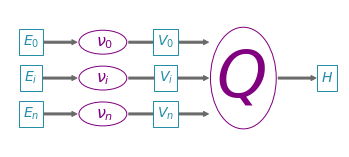
\includegraphics[width=1\textwidth]{../paper/figures/path_of_q.png}
    \end{figure}
\end{frame}


\subsection{Measurement Specification $\vtotalc$}

\begin{frame}<presentation:1|handout:1>{Typed Measurable Visual Components: $\vtotalc$}
    \begin{columns}
        \column{0.31\textwidth}
        \begin{equation*}
            \begin{tikzcd}[ampersand replacement=\&, row sep=huge]
                \onslide*<1|handout:1>{\vfiberc}
                \onslide*<1|handout:1>{\arrow[r, hook]} \& 
                \onslide*<1|handout:1>{\vtotalc} 
                \onslide*<1|handout:1>{\arrow[d, "\pi"']} \\
                \& 
                \onslide*<1|handout:1>{\dbasec} 
                \onslide*<1|handout:1>{\arrow[u, "\vsectionc \in \cgamma{\opensetc}{\vtotalc\restriction_{\opensetc}}"', bend right, pos=.5]}
            \end{tikzcd}
        \end{equation*}
        \column{0.69\textwidth}
    \only<1|handout:1>{
        \begin{description}[style=nextline]
            \item[\textcolor{total}{Data \vtotalc}]{continuity + visual fields}
            \item[\textcolor{base}{Continuity \dbasec}]{data continuity}
            \item[\textcolor{fiber}{components \vfiberc}] {visual components \cite{bertinIIPropertiesGraphic2011} of a graphic, e.g. x and y position, area, color, line thickness}
        \end{description}
        }
    \end{columns}
    \pause 
    \only<1|handout:1>{
        \begin{alertblock}{}
            \begin{description}[style=nextline]
                \item[\textcolor{section}{visual components}]{$\cgamma{\opensetc}{\vtotalc\restriction_{\opensetc}} \coloneqq \big\{\vsectionc: \opensetc\rightarrow \vtotalc\restriction_{\opensetc} \; \bigm{\vert} \pi(\vsectionc(\dbasepointc)) = \dbasepointc\;for\, all\; \dbasepointc \in \opensetc \big\}$}
            \end{description}
        \end{alertblock}
    }
\end{frame}

\begin{frame}<presentation:1|handout:1>
    \frametitle{Transformations in Data $\vchannelc: \dsectionc \mapsto \vsectionc$}
    %rewrite in gamma notation
    \begin{figure}
        \includegraphics[.35\textwidth]{figures/math/nu_table.png}
    \end{figure}
    Given $\dsectionc(\dbasepointc) = \dsectionc(\dfunchc(\dbasepointc^{\prime}))$ and  $\vsectionc(\dbasepointc) = \vsectionc(\dfunchc(\dbasepointc^{\prime}))$
    \begin{description}
        \item[equivariance] $\dfunctc_{\vtotalc}(\vchannelc_{\opensetc}(\dsectionc))
        = \vchannelc_{\opensetc}(\dfunctc_{\dtotalc}(\dsectionc))$, $\vchannelc_{\opensetc} = {\vchannelc^{\prime}}_{\opensetc^{\prime}}$
        \item[continuity] $\lim\limits_{x\to \dbasepointc}(\vchannelc(\dsectionc(x))) = \vchannelc(\dsectionc(\dbasepointc))$ for all $\dbasepointc \in \dbasec$ 
    \end{description}
\end{frame}  

\begin{frame}{Data to Visual Transformation $\vchannelc: \dfiberc_{\dbasepointc} \mapsto \vfiberc_{\dbasepointc}$}
    %remove maps to 
$\pi(\dtotalc) = \pi(\vchannelc(\dtotalc))$ and $\vchannelc$ is composable s.t 
    \begin{columns}
        \column{.15\textwidth}
        \begin{equation*}
        \begin{tikzcd}[ampersand replacement=\&]
            \dfiberc_{\dbasepointc} 
            \arrow[rr, "\vchannelc"] 
            \arrow[dd, "\dfunctc_{\dtotalc}"'] 
            \& \& 
            \vfiberc_{\dbasepointc} 
            \arrow[dd, "\dfunctc_{\vtotalc}"] \\
            {} 
            \arrow[rr, dashed]
            \& \& {} \\
            {\dfiberc^{\prime}}_{\dbasepointc} 
            \arrow[rr, "\vchannelc^{\prime}"']
            \& \& 
            {\vfiberc^{\prime}}_{\dbasepointc}
            \end{tikzcd}
        \end{equation*}
        \column{.5\textwidth} 
        \begin{equation*}
        \begin{tikzcd}[ampersand replacement=\&, row sep=huge]
            \dfiberc_{\dbasepointc} 
            \arrow[rr, "\vchannelc_{\dtotalc} ", color=artist] 
            \arrow[rrdd, "{\vchannelc_{\dtotalc,\vtotalc}}" description, dashed, color=artist] 
            \&  \& 
            \vfiberc_{\dbasepointc}\coloneqq {\dfiberc_{\dbasepointc}}^{\vtotalc} 
            \arrow[dd, "\vchannelc_{\vtotalc}", color=artist] \\
            \& \& \\
            \&  \& {\vfiberc_{\dbasepointc}}^{\vtotalc}
            \end{tikzcd}
        \end{equation*}
    \end{columns}
    
\end{frame}

\begin{frame}<presentation:1|handout:1>\frametitle{$\vchannelc:\dfuncc_{\dtotalc} \rightarrow \dfuncc_{\vtotalc}$: Stevens' Scales \cite{stevensTheoryScalesMeasurement1946}}
    \begin{table}[H]
        \begin{tabularx}{\textwidth}{|l|l|X|}\toprule
            \textbf{scale} & \textbf{group} & \textbf{constraint} \\\midrule
            nominal & permutation &  $\text{if } \delement_1 \neq \delement_2 \text{ then } \vchannel (\delement_1) \neq\vchannel(\delement_2)$\\
            ordinal &  monotonic & $\text{if } \delement_1 \leq \delement_2 \text{ then } \vchannel (\delement_1) \leq \vchannel(\delement_2)$\\
            interval &  translation &  $\vchannel (\delement + c) = \vchannel(\delement) + \vchannel(c)$ \\
            ratio &  scaling &  $\vchannel(\delement* c) = \vchannel(\delement)*\vchannel(c) $\\ \bottomrule
        \end{tabularx}
    \end{table}
\end{frame}


\begin{frame}<presentation:1|handout:1>
    \frametitle{Shared Components: $\vchannelc = \prod\limits_{i=0}^{n}\vchannelc_i$}
    \begin{equation}
        \begin{tikzcd}[ampersand replacement=\&]
            \dfiberc_a\times \dfiberc_b 
            \arrow[rr, "\vchannelc", color=artist] 
            \arrow[rd, "p_{\dfiberc}", color=fiber] \& \& \vfiberc_a\times \vfiberc_b 
            \arrow[rd, "p_{\vfiberc}", color=fiber] \& \\    \& 
            \dfiberc_{a} 
            \arrow[rr, "\vchannelc_{a}", dashed, color=artist] \& \& \vfiberc_a \\
            \dfiberc_a\times \dfiberc_c 
            \arrow[rr, "\vchannelc^{\prime}", color=artist] 
            \arrow[ru, "p_{\dfiberc^{\prime}}"', color=fiber] \& \& 
            {\vfiberc_a}^{\prime}\times {\vfiberc_c}^{\prime} 
            \arrow[ru, "p_{\vfiberc^{\prime}}"', color=fiber] \&           
            \end{tikzcd}
    \end{equation}
    \begin{alertblock}{Consistent Transformations \cite{hullmanKeeping2018}}
        if $p_{\dfiberc} = p_{\dfiberc^{\prime}}$ then $p_{\vfiberc}(\vchannelc(\dsectionc)) = p_{\vfiberc^{\prime}}(\vchannelc^{\prime}(\dsectionc^{\prime}))$ s.t. there exists a transformation $\vchannelc_a: \dfiberc_{a}\rightarrow \vfiberc_{a}$
    \end{alertblock}
\end{frame}


\subsection{Combining Components into Visualizations}
\begin{frame}<presentation:1|handout:1>{Assembly $\vmarkc$}
    \begin{equation*}
        \begin{tikzcd}[ampersand replacement = \&]
            \cgamma{\opensetc}{\vtotalc\restriction_{\opensetc}} 
            \arrow[rrrr, "\vmarkc", color=artist] 
            \arrow[ddd, "\dfunctc_{\vtotalc} \circ \dfuncpullc_{\vtotalc}"', color=action] 
            \& \& \& \& 
            \imartist{\opensetgc}{\gtotalc\restriction_{\opensetgc}} 
            \arrow[ddd, "\dfunctc_{\gtotalc} \circ \dfuncpullc_{\gtotalc}", dotted, color=action]  \\
            \& 
            \opensetc 
             \&  \& 
            \opensetgc 
            \arrow[ll, "\vindexc"', color=functor]   \& \\
            \& 
            \opensetc^{\prime} 
            \arrow[u, "\dfunchc_{\dtotalc}", color=action] 
            \&  \& 
            \opensetgc^{\prime} 
            \arrow[ll, "\vindexc"', color=functor] 
            \arrow[u, "\dfunchc_{\gtotalc}"', dotted, color=action] 
            \& \\
            \cgamma{\opensetc^{\prime}}{\vtotalc^{\prime}\restriction_{\opensetc^{\prime}}}
            \arrow[rrrr, "\vmarkc^{\prime}", color=artist] 
            \& \&  \& \& 
            \imartist{\opensetgc^{\prime}}{\gtotalc^{\prime}\restriction_{\opensetgc^{\prime}}}
            \end{tikzcd}
        \end{equation*}
    \begin{alertblock}{equivariance}
       \begin{equation*}
        \vmarkc^{\prime}(\dfunctc_{\vtotalc}(\vsectionc(\dfunchc_{\dtotalc}(\vindexc(\gbasepointc^{\prime}))))) = \dfunctc_{\gtotalc}(\vmarkc(\vsectionc(\vindexc(\dfunchc_{\gtotalc}(\gbasepointc^{\prime})))))
       \end{equation*}
    \end{alertblock}
\end{frame}

\begin{frame}<presentation:1|handout:1>{Components to Graphic}
    \begin{figure}
        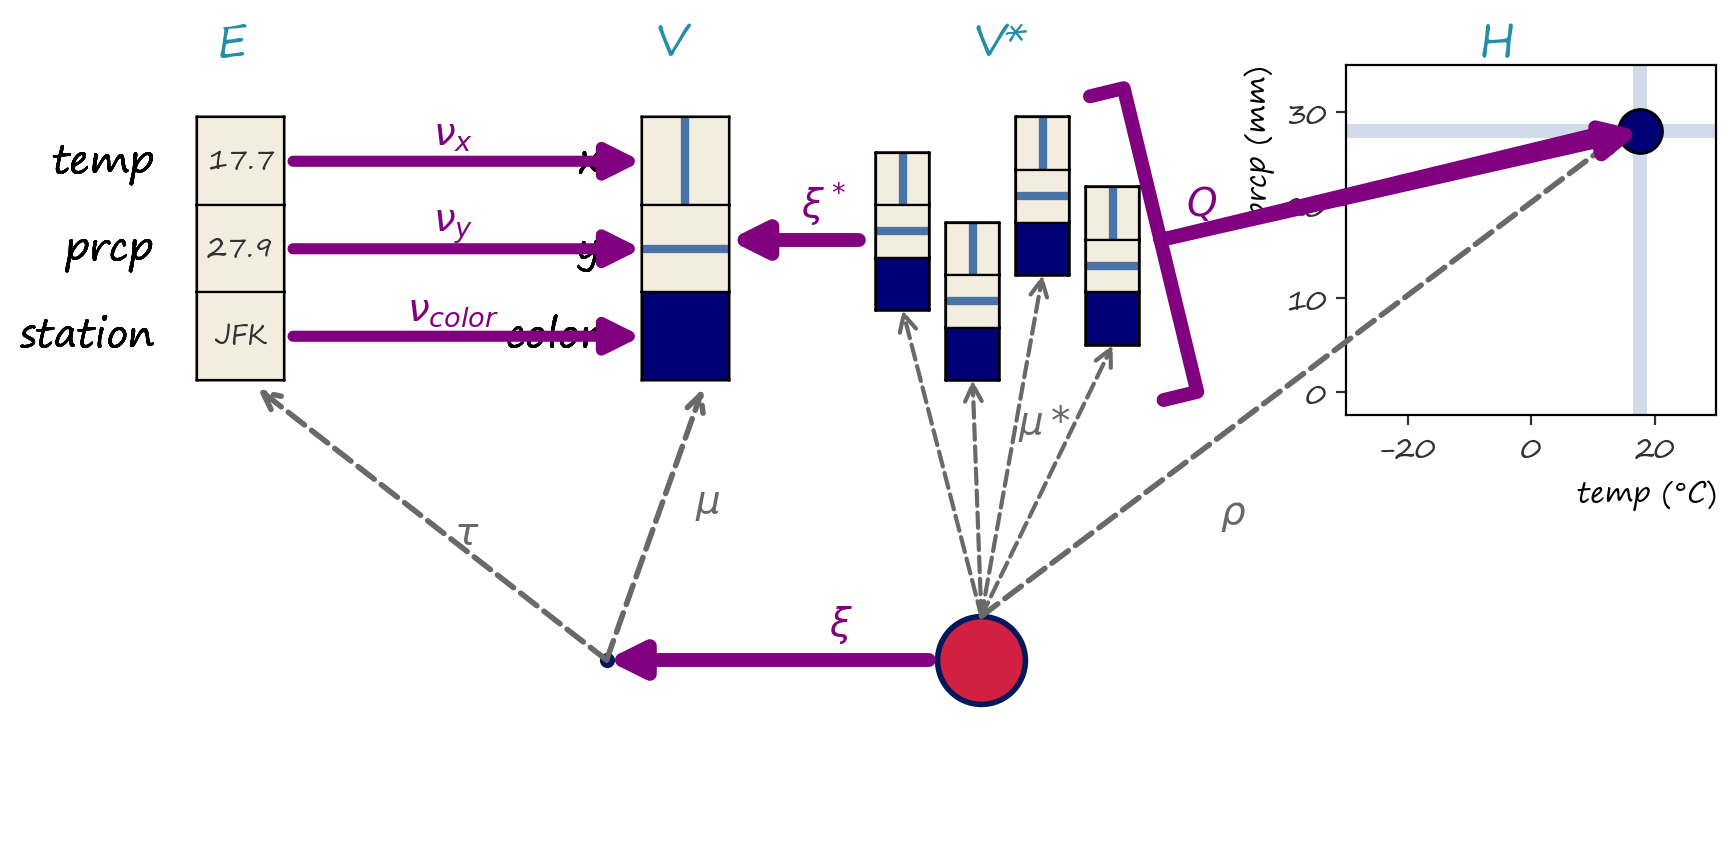
\includegraphics[scale=.15]{../paper/figures/qhat.png}
    \end{figure}
\end{frame}

\begin{frame}<presentation:1|handout:1>{Implementation Choices: $\vartistc_{\dbasec} = \vartistc_{\gbasec}$}
    \begin{figure}
        \includegraphics[scale=.5]{figures/math/implement_paths).png}
    \end{figure}
\end{frame}

\begin{frame}{Combining Qs}
    The codomain of all $\vmarkc$ targeting the same output space is the bundle $\gtotalc$ and $Hom(\gbasec_1, \gtotalc) + Hom(\gbasec_2, \gtotalc) = Hom(\gbasec_1 + \gbasec_2, \gtotalc)$; therefore 
    $\sqcup \vmarkc_i(\cgamma{\opensetc_i}{\dtotalc_i\restriction_{\opensetc_i}}) = \cgamma{\sqcup \opensetgc_i}{\gtotalc\restriction_{\sqcup\opensetgc_i}}$
    \begin{figure}
        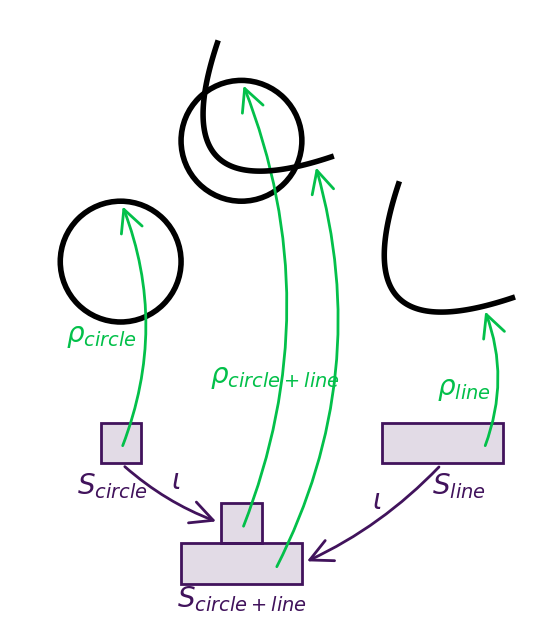
\includegraphics[scale=.25]{figures/math/qcom.png}
    \end{figure}
\end{frame}

\begin{frame}{Compatible Qs}
    \includegraphics[scale=.5]{figures/math/compatiblw_q.png}
\end{frame}
\end{document}